% THIS IS SIGPROC-SP.TEX - VERSION 3.1
% WORKS WITH V3.2SP OF ACM_PROC_ARTICLE-SP.CLS
% APRIL 2009
%
% It is an example file showing how to use the 'acm_proc_article-sp.cls' V3.2SP
% LaTeX2e document class file for Conference Proceedings submissions.
% ----------------------------------------------------------------------------------------------------------------
% This .tex file (and associated .cls V3.2SP) *DOES NOT* produce:
%       1) The Permission Statement
%       2) The Conference (location) Info information
%       3) The Copyright Line with ACM data
%       4) Page numbering
% ---------------------------------------------------------------------------------------------------------------
% It is an example which *does* use the .bib file (from which the .bbl file
% is produced).
% REMEMBER HOWEVER: After having produced the .bbl file,
% and prior to final submission,
% you need to 'insert'  your .bbl file into your source .tex file so as to provide
% ONE 'self-contained' source file.
%
% Questions regarding SIGS should be sent to
% Adrienne Griscti ---> griscti@acm.org
%
% Questions/suggestions regarding the guidelines, .tex and .cls files, etc. to
% Gerald Murray ---> murray@hq.acm.org
%
% For tracking purposes - this is V3.1SP - APRIL 2009

\documentclass{acm_proc_article-sp}
\usepackage[none]{hyphenat}
\usepackage{graphicx}

\begin{document}

\title{Detecting and Combating ARP Spoofing}
%
% You need the command \numberofauthors to handle the 'placement
% and alignment' of the authors beneath the title.
%
% For aesthetic reasons, we recommend 'three authors at a time'
% i.e. three 'name/affiliation blocks' be placed beneath the title.
%
% NOTE: You are NOT restricted in how many 'rows' of
% "name/affiliations" may appear. We just ask that you restrict
% the number of 'columns' to three.
%
% Because of the available 'opening page real-estate'
% we ask you to refrain from putting more than six authors
% (two rows with three columns) beneath the article title.
% More than six makes the first-page appear very cluttered indeed.
%
% Use the \alignauthor commands to handle the names
% and affiliations for an 'aesthetic maximum' of six authors.
% Add names, affiliations, addresses for
% the seventh etc. author(s) as the argument for the
% \additionalauthors command.
% These 'additional authors' will be output/set for you
% without further effort on your part as the last section in
% the body of your article BEFORE References or any Appendices.

\numberofauthors{4} %  in this sample file, there are a *total*
% of EIGHT authors. SIX appear on the 'first-page' (for formatting
% reasons) and the remaining two appear in the \additionalauthors section.
%
\author{
% You can go ahead and credit any number of authors here,
% e.g. one 'row of three' or two rows (consisting of one row of three
% and a second row of one, two or three).
%
% The command \alignauthor (no curly braces needed) should
% precede each author name, affiliation/snail-mail address and
% e-mail address. Additionally, tag each line of
% affiliation/address with \affaddr, and tag the
% e-mail address with \email.
%
% 1st. author
\alignauthor
Chai Ming Xuan\\
       \affaddr{National University of Singapore}\\
       \email{mingxuan@u.nus.edu}
% 2nd. author
\alignauthor
Er Xue Hui\\
       \affaddr{National University of Singapore}\\
       \email{xuehuier@u.nus.edu}
% 3rd. author
\alignauthor 
Wu Wenqi\\
       \affaddr{National University of Singapore}\\
       \email{wenqi.wu@u.nus.edu}
\and  % use '\and' if you need 'another row' of author names
% 4th. author
\alignauthor Zhu Chunqi\\
       \affaddr{National University of Singapore}\\
       \email{chunqi@u.nus.edu}
}
\maketitle
\begin{abstract}
In light of the 'Sparkle Vulnerability'\footnote{https://sparkle-project.org/documentation/security/} incident that occurred earlier this year, our team has been particularly interested in preventing man-in-the-middle (MITM) attacks. We realised that such attacks are easy to carry out and are quite common as well. Eventually, we decided to focus on preventing ARP Spoofing, a means which allows the attacker to carry out such MITM attacks. 

Since the early days of the computer, the ARP cache has been an easy target for ARP attacks like ARP spoofing. Even until today, it is still relatively easy to carry out an ARP spoof, and it remains rather difficult to defend against it. 

Thus, our project aims to create a program for users to actively detect if they are victims of ARP spoofing, and to offer alternative ways to protect themselves over an unsecure network.
\end{abstract}

% A category with the (minimum) three required fields
\category{C.2.0}{Computer-Communication Networks}{General - Data Communications, Security and Protection}

%A category including the fourth, optional field follows...
\category{D.4.6}{Security and Protection}{Authentication,\\ Verification}

\terms{Network Security, Intrustion Detection System (IDS), \\
Address Resolution Protocol (ARP), spoofing}

\keywords{ARP spoofing, ARP Poisoning, network security, attack, MITM,
IDS, ARP protection}

\section{Introduction}
The Address Resolution Protocol (ARP) is an important protocol in computer network communications. \\ Without this protocol, it would be difficult for computers to \\communicate with each other, because we would not know the MAC address of the computer we are communicating with. Thus, it would be difficult to establish an IP-to-MAC address mapping.

However, it is also one of the easier protocols to spoof and carry out attacks on, because of the lack of viable solutions to protect the ARP cache. In fact, such attacks are easy to carry out over a wireless network if it is not protected by WPA-Enterprise encryption. Over a Local Area Network (LAN), such attacks require a wiretap if the network uses switches instead of hubs. 

Some common attacks that can occur after an ARP Spoof are man-in-the-middle (MITM), Denial-of-Service (DOS), or even session hijacking. 
In such cases, the security principles of Confidentiality, Integrity and Availability may be violated. 
We will be illustrating how an ARP Spoof occurs in Section 2. 

Some common programs which users can use to carry out such an attack include `Ettercap' and `Cain and Abel'. As these programs are open source, almost anyone can easily carry out ARP Spoofing with some basic technical knowledge. 


\section{Background}
In order to understand how ARP spoofing occurs, we will need to cover the basics on how computers communicate with each other. In this section, we will be explaining how computers do so, and introduce the basic notions of how an ARP spoof is carried out. 

\subsection{Models and Abstractions}
In computer networking, the communication protocols are categorised and organised into different layers. In the TCP/IP Model, there are 5 layers of abstraction: 

1. Application Layer\\
2. Transport Layer\\
3. Internet Layer\\
4. Link Layer\\
5. Physical Layer\\

DHCP is an application layer protocol and ARP is a link layer protocol.

In the OSI Model, there are 7 layers of abstraction:

7. Application Layer \\
6. Presentation Layer \\
5. Session Layer \\
4. Transport Layer \\
3. Network Layer \\
2. Data Link Layer \\
1. Physical Layer 

(show picture of comparison between both models?) 

\subsection{Computer Communications}
In a typical modern computer, all IP addresses are resolved dynamically through the use of the Dynamic Host \\Configuration Protocol (DHCP). This is carried out in the following steps: \\

1. DHCP Discover: \\
The new host broadcasts a DHCP discover message, where 255.255.255.255 is a typical broadcast address.  

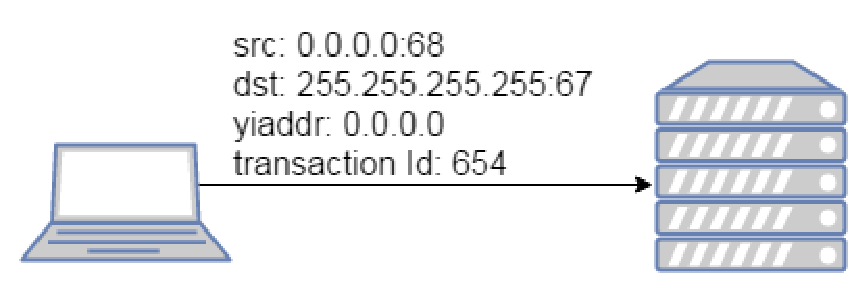
\includegraphics[width=3in]{DHCP_Discover.eps}

2. DHCP Offer: \\
The DHCP server responds with a DHCP offer. 

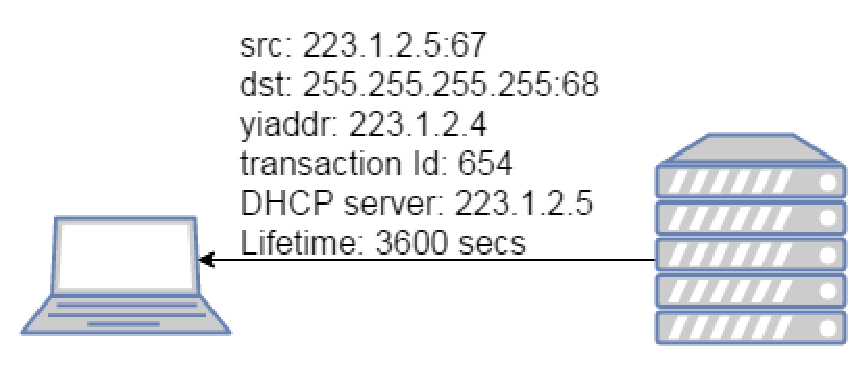
\includegraphics[width=3in]{DHCP_Offer.eps}

3. DHCP Request: \\
The host selects from the offers and sends a DHCP request. 

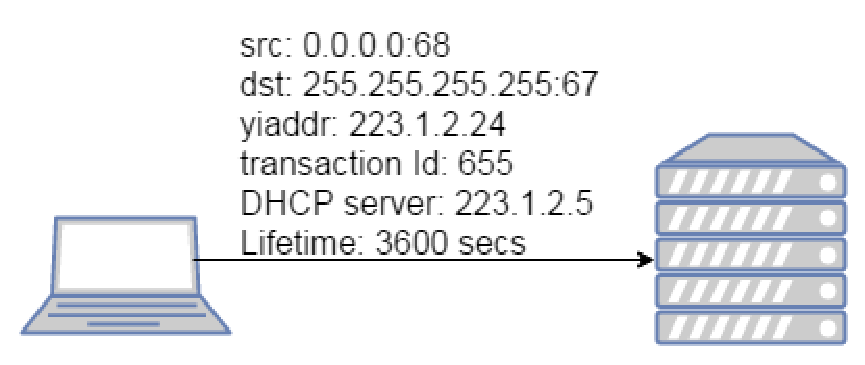
\includegraphics[width=3in]{DHCP_Request.eps}

4. DHCP ACK: \\ 
The DHCP Server confirms the requested parameters. 

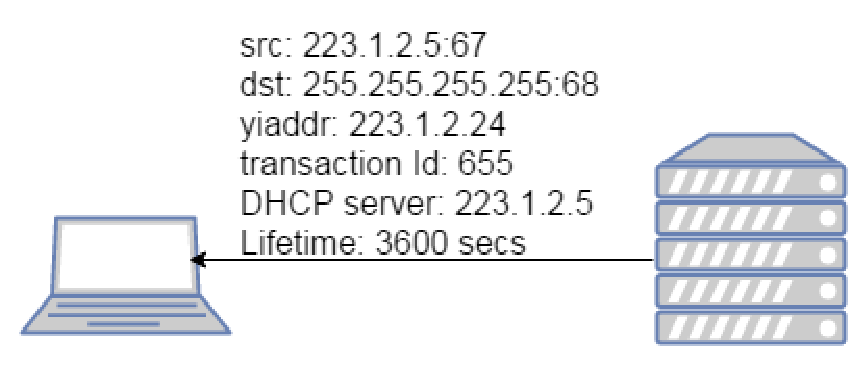
\includegraphics[width=3in]{DHCP_Ack.eps}


After that, assuming everyone has already had their IPs assigned to them via DHCP, suppose the the user Alice wishes to send some information to Bob. The following steps are then carried out: 

1. ARP Request: Alice's computer sends out an ARP request to find out which MAC address has Bob's IP. 

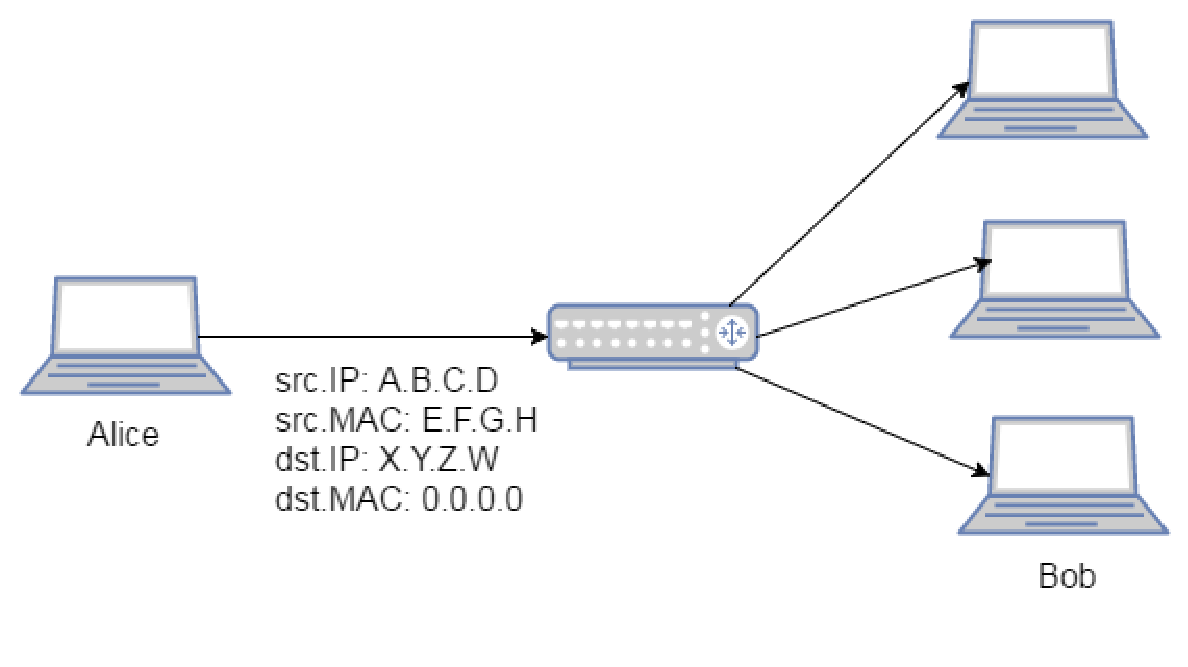
\includegraphics[width=3in]{ARP_Request.eps}

2. When Bob's computer receives the request, he sends back an ARP response packet. 

\includegraphics[width=3in]{ARP_Response.eps}

3. Alice gets the response and stores the corresponding IP-to-MAC entry into the ARP cache. 


\subsection{Poisoning the ARP Cache}
There are 3 main ways to poison the ARP cache. The first is to send a broadcast request, the second is to send multiple responses, and the third is an unsolicited response. In this paper, we will only cover the second method as it is more commonly used.

If an attacker, Eve, wishes to carry out ARP spoofing, this is typically what happens: 

1. Alice's computer sends out an ARP request to find out what is Bob's MAC address. 

2. Before Bob's computer can reply, the attacker, Eve, sends a spam of packets to Alice's computer, claiming to be Bob. The ARP cache then becomes poisoned. 

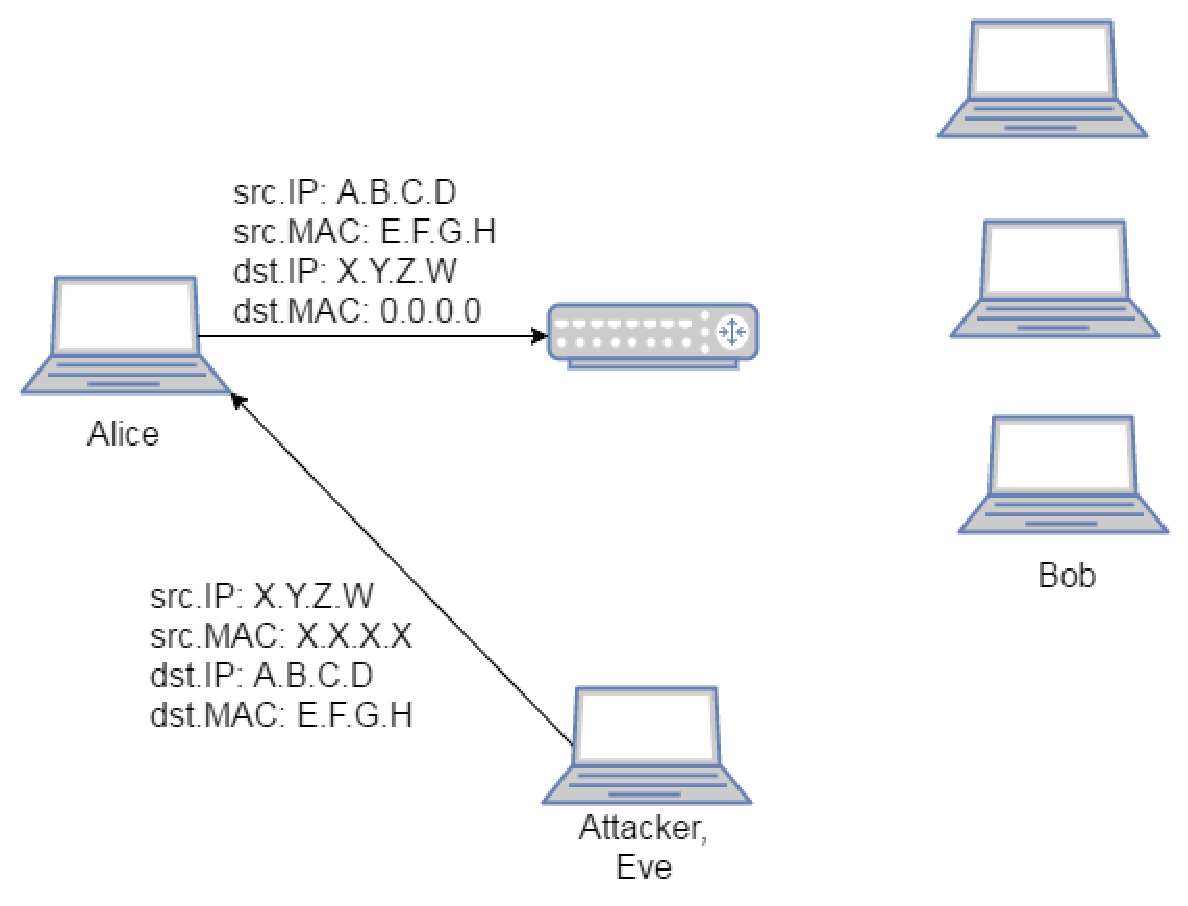
\includegraphics[width=3in]{Poisoned_ARP.eps}

In this case, there is a race condition between Eve and Bob to send a response to Alice. If Eve succeeds in responding to Alice before Bob can do so, Alice's ARP cache becomes successfully poisoned. 

\section{Current Solutions and \\Mitigations}
There are currently many solutions in the market to combat ARP Spoofing. However, many of these solutions are described to have major issues. From \cite{vivek:arp}, \cite{navid:arp2} and \cite{goldendeep:arp3},  these are the summaries and drawbacks of current implementations in the market:

1. Use of Cryptographic Techniques \\
Examples: S-ARP \\
This method suggests that the ARP protocol be redesigned with cryptographic measures in place. However, implementing such cryptographic measures severely degrades the runtime performance of the ARP protocol. 

2. Passive Detection \\
Examples: Agnitum Outpost Firewall\\
Such methods only detect ARP spoofing but are unable to do anything to correct it. 

3. Kernel-based patches\\
Examples: Anticap, Antidote \\
A patch is given to fix the OS Kernel. However, this may cause compatibility issues. 

4. Making ARP entries static\\ 
In this method, ARP entries are configured to be static. In this case, DHCP will not be used to resolve local IP addresses for a computer. However, it will not be very user-friendly for standard office workers to configure, and will be very difficult for network administrators to manage IP-to-MAC mappings in a huge company. 


\section{Goals}
In taking up this project, we hoped to achieve the following goals: 

1. Provide users with a means to actively combat ARP spoofing \\
2. Make any network more secure. \\
3. Provide a GUI for users to see what is happening in their network in real-time. 

\section{Proof of Concept}
\subsection{Implementation System}
Operating System: \\
OSX El Capitan, Arch-Linux [Manjaro 15.12 Capella]

Software: \\
Python 2.7 with the following libraries: scipy, scapy, \\matplotlib, tkinter, numpy \\ Ettercap \\ Wireshark

\subsection{Assumptions}
1. Attacker's computer has a normal network stack. 

2. Victim computer has at least one TCP port open.

3. All devices have a TCP/IP network stack up and running.

4. Attacker only modifies his data in the Ethernet layer. If he modifies his data in the Network layer as well, then we would not be able to determine who the attacker is, although we can detect that it is an ARP spoof based on the volume of packets sent. 

\subsection{Overall Architecture}
put a summary of the software system here.

\subsection{The Attacker}
In our solution, we used Ettercap to stimulate an ARP Spoofing attack. 

\subsection{The Defender Module}

(ming xuan's code) 

\subsection{The Spoof Detection Engine (IDS)}

(wenqi's code)

\subsection{The GUI}

to insert a picture once GUI is completed

\section{Our solution versus current \\solutions}
In contrast to current available solutions, we tried to adopt an active method of detecting ARP spoofing. 

\section{Limitations and Future Work}
Our project has several flaws which we were unable to resolve within a reasonable timeframe: 

1. Our solution will not work on a network that employs WPA-Enterprise level of encryption. This is because the structure of WPA-Enterprise is such that each user can only see his incoming or outgoing network connections. 

2. Our solution assumes that the user does not have any form of defence installed on his computer. (eg. no firewall that can prevent ARP spoofing, a network that does not use any enterprise level encryption, etc.) 

3. The attacks have only been tested to work for various users across the wireless network which uses no encryption, WEP, WPA, and WPA2. While it might work on a network that uses a hub, it might require a wiretap for a switched network.  

We hope to improve our solution for a more varied set of systems in the future. 

\section{Conclusion}
Through this project, we have learnt that ARP Spoofing is not easy to defend against. Even though there are solutions on the market that have been out for a while, unless one is using a network encrypted by WPA-Enterprise, it is otherwise easy to fall prey to such attacks. 

Furthermore, as active detection of ARP spoofing is not widely implemented yet, our solution may not be entirely foolproof. Thus, we will need to put in more work to make the solution more viable for a wider variety of situations. 

(to modify conclusion and include more stuff) 
%\end{document}  % This is where a 'short' article might terminate

%ACKNOWLEDGMENTS are optional
\section{Acknowledgements}
First and foremost, we would like to thank Prof. Hugh Anderson for his guidance and patience with us throughout the semester. Our initial project was to investigate the hacking of Hello Barbie. However, we eventually decided to change the topic for various reasons, and he very kindly allowed us to do so. This is despite the topic being self-proposed and changed quite late in the semester. 

Our thanks also goes out to him for loaning us the Hello Barbie even though we eventually dropped the project. 

In addition, our appreciation also goes out to our friends who have loaned us various items for our project, such as a DLink Dir-825 router which runs on DD-RWT, so that we could work on the project in school. 

%
% The following two commands are all you need in the
% initial runs of your .tex file to
% produce the bibliography for the citations in your paper.
\bibliographystyle{abbrv}
\bibliography{sigproc}  % sigproc.bib is the name of the Bibliography in this case
% You must have a proper ".bib" file
%  and remember to run:
% latex bibtex latex latex
% to resolve all references
%
% ACM needs 'a single self-contained file'!
%

\newpage

\subsection{Tables}
Because tables cannot be split across pages, the best
placement for them is typically the top of the page
nearest their initial cite.  To
ensure this proper ``floating'' placement of tables, use the
environment \textbf{table} to enclose the table's contents and
the table caption.  The contents of the table itself must go
in the \textbf{tabular} environment, to
be aligned properly in rows and columns, with the desired
horizontal and vertical rules.  Again, detailed instructions
on \textbf{tabular} material
is found in the \textit{\LaTeX\ User's Guide}.

Immediately following this sentence is the point at which
Table 1 is included in the input file; compare the
placement of the table here with the table in the printed
dvi output of this document.

\begin{table}
\centering
\caption{Frequency of Special Characters}
\begin{tabular}{|c|c|l|} \hline
Non-English or Math&Frequency&Comments\\ \hline
\O & 1 in 1,000& For Swedish names\\ \hline
$\pi$ & 1 in 5& Common in math\\ \hline
\$ & 4 in 5 & Used in business\\ \hline
$\Psi^2_1$ & 1 in 40,000& Unexplained usage\\
\hline\end{tabular}
\end{table}

To set a wider table, which takes up the whole width of
the page's live area, use the environment
\textbf{table*} to enclose the table's contents and
the table caption.  As with a single-column table, this wide
table will ``float" to a location deemed more desirable.
Immediately following this sentence is the point at which
Table 2 is included in the input file; again, it is
instructive to compare the placement of the
table here with the table in the printed dvi
output of this document.


\begin{table*}
\centering
\caption{Some Typical Commands}
\begin{tabular}{|c|c|l|} \hline
Command&A Number&Comments\\ \hline
\texttt{{\char'134}alignauthor} & 100& Author alignment\\ \hline
\texttt{{\char'134}numberofauthors}& 200& Author enumeration\\ \hline
\texttt{{\char'134}table}& 300 & For tables\\ \hline
\texttt{{\char'134}table*}& 400& For wider tables\\ \hline\end{tabular}
\end{table*}
% end the environment with {table*}, NOTE not {table}!


\begin{figure*}
\centering
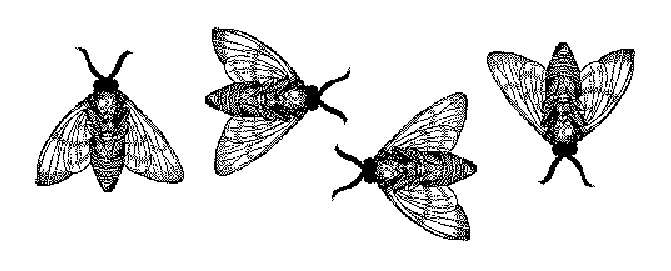
\epsfig{file=flies.eps}
\caption{A sample black and white graphic (.eps format)
that needs to span two columns of text.}
\end{figure*}
%ending with figure* is for images that span 2 cols 
 


\end{document}
